\subsection{Progettazione architetturale}
\textit{\textbf{Periodo}: dal 2021-01-18 al 2021-03-08}

L'inizio di questa fase coincide con data della revisione dei requisiti e conclude con la scadenza della revisione di progettazione.

\subsubsection{Attività}

\begin{itemize}
\item \textbf{Incremento e verifica documenti}: ;
\item \textbf{Technology baseline}: ;
\item \textbf{Consolidamento}: viene realizzata la presentazione da esporre in sede di revisione di progettazione e si approfondiscono aspetti lacunari riguardo il progetto.
\end{itemize}

\subsubsection{Periodi}

\begin{itemize}
\item \textbf{Periodo 1}: \textit{dal 2021-01-18 al 2021-01-31}. \\
Correzione;
\item \textbf{Periodo 2}: \textit{dal 2021-01-31 al 2021-03-01}. \\
Technology baseline;
\begin{itemize}
\item \textbf{Incremento 1}: \textit{dal 2021-02-04 al 2021-02-09};
\item \textbf{Incremento 2}: \textit{dal 2021-02-09 al 2021-02-14};
\item \textbf{Incremento 3}: \textit{dal 2021-02-14 al 2021-02-19};
\item \textbf{Incremento 4}: \textit{dal 2021-01-19 al 2021-02-24}.
\end{itemize}
\item \textbf{Periodo 3}: \textit{dal 2021-03-01 al 2021-03-08}. \\
Viene svolta l'attività di consolidamento. Il periodo conclude con la consegna del materiale relativo alla revisione dei requisiti;
\end{itemize}

\subsubsection{Diagramma di Gantt}

\begin{figure}[H]
\centering

\centerline{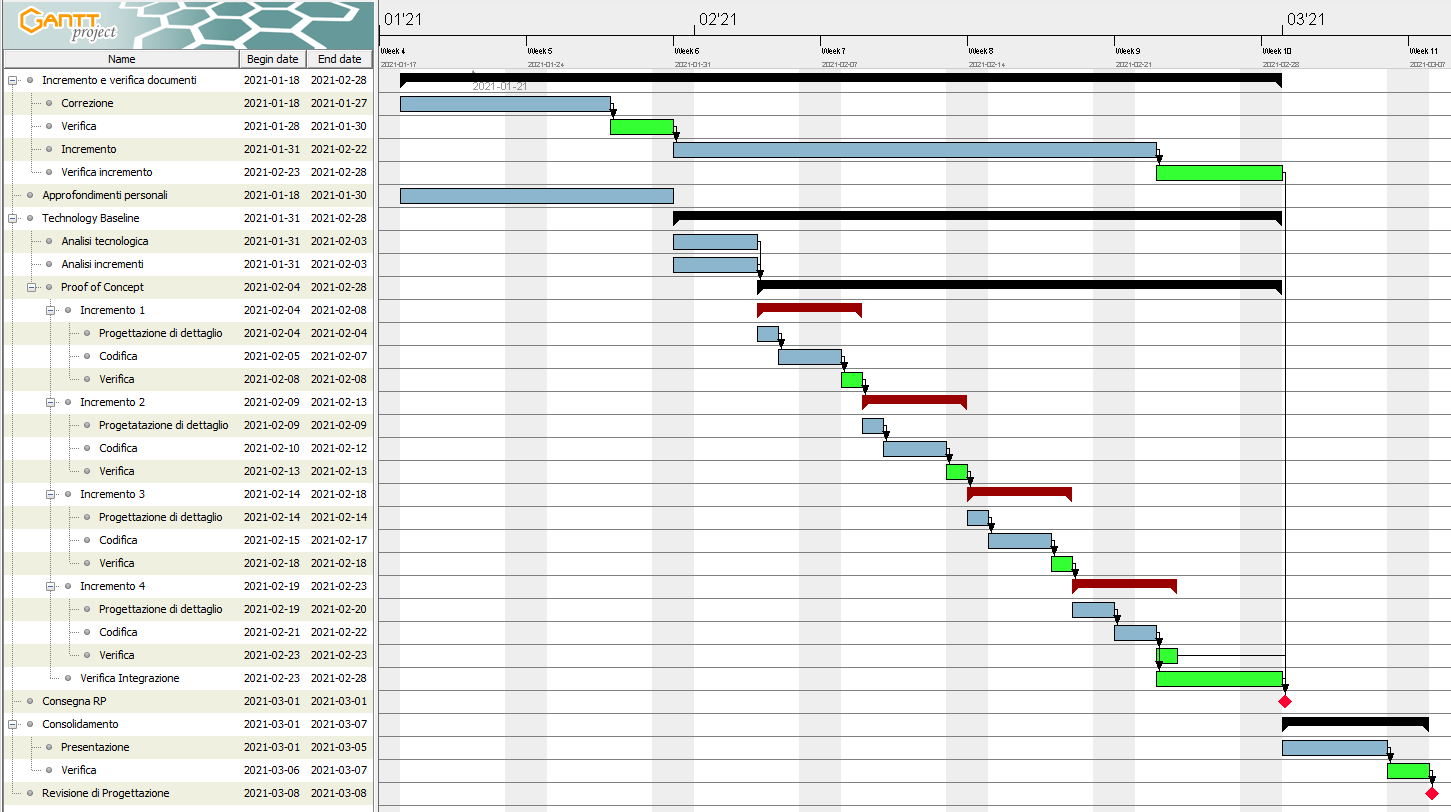
\includegraphics[scale=0.5]{res/Pianificazione/Gantt/progettazione}}
\caption{Diagramma di Gantt per il periodo di progettazione}
\end{figure}